\chapter{Implementierung} \label{chap:implementierung}

Nachdem im Letzten Kapitel (siehe \autoref{chap:Konzept}) das Konzept der Lösung der Aufgabenstellung beschrieben wurde, wird in diesem Kapitel die Implementierung der Software beschrieben.
Ziel ist es alle beschriebenen Aufgabenteile in Python umzusetzen und eine Software zu entwickeln, die in der Lage ist, die Anforderungen der Aufgabenstellung zu erfüllen. Ausschnitte aus dieser Software sind im Kapitel des Konzepts bereits beschrieben und werden hier weiter ausgeführt.

Die Implementierung erfolgt in mehreren Schritten:

\begin{enumerate}
    \item \textbf{Umzug auf lokale Programmierung} 
    \item \textbf{Einpflegen der JSON Parameter} 
    \item \textbf{Entwicklung der API} 
    \item \textbf{Installation im Labor}

\end{enumerate}

In den folgenden Kapiteln werden die einzelnen Schritte genauer beschrieben.

\section{Umzug auf lokale Programmierung} \label{subsec:umzug_auf_lokale_programmierung}

Die Struktur dieser Implementierung folgt der Konzeption der Programmstruktur nach dem MVC-Prinzip \autoref{fig:MVC_struktur}, welches in \autoref{sec:architektur} beschrieben ist.
Dieses Modell Trennt die Datenverarbeitung, die Darstellung und die Steuerung der Software in drei verschiedene Module auf.
Die Datenverarbeitung wird in einem eigenen Modul abgetrennt, Darstellung und Steuerung sind in der API zusammengefasst.

Das Pycore Modul, welches diese benötigten, selbst entwickelten, Bibliotheken zur Verfügung stellt, ist auch in \autoref{fig:Projektstruktur} als eigener Ordner mit Python Skripten in seinen Unterverzeichnissen dargestellt. Es beinhaltet die Funktionen, welche den Datensatz aufbereiten und dem Neuronalen Netzwerk zum Training zur Verfügung stellen.
Die wichtigsten Bestandteile sind die Konvertierung in Graustufen, die Aufteilung des Datensatzes in Trainings- und Testdaten, sowie der Download des untrainierten neuronalen Netzwerks und dessen parametrisierung bezüglich der Klassifikationsaufgabe.

\begin{figure}[H]
    \centering
    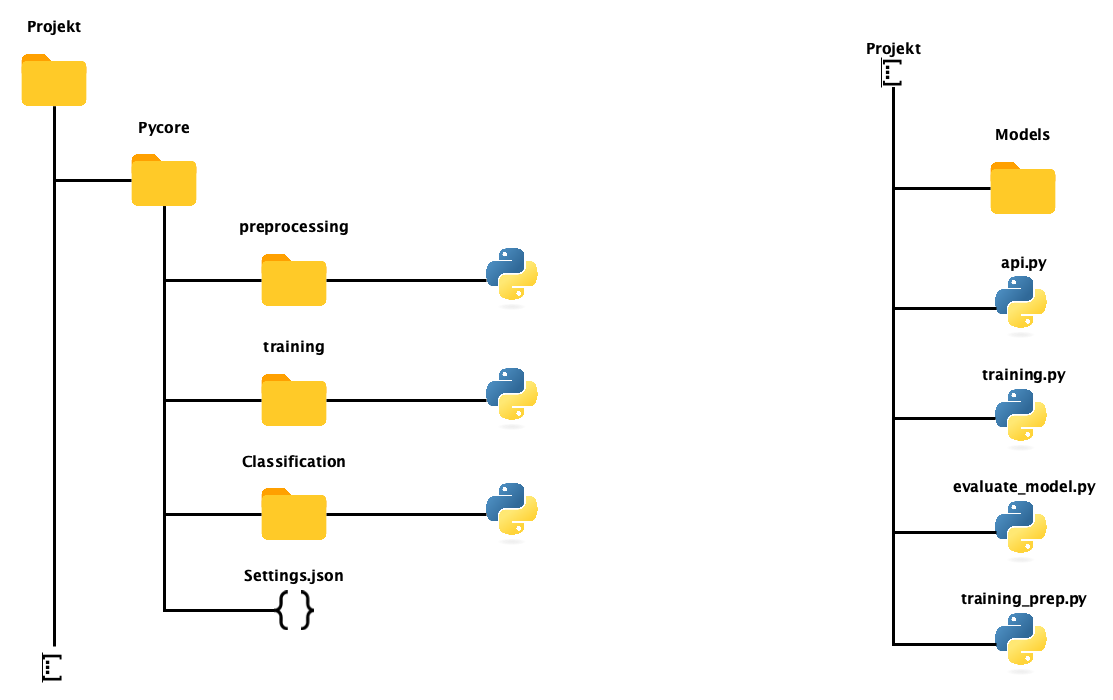
\includegraphics[width=0.8\textwidth]{Projektstruktur.png}
    \caption{Projektstruktur der Software im Dateiverzeichnis}
    \label{fig:Projektstruktur}
\end{figure}

Die in der Grafik \autoref{fig:Projektstruktur} dargestellte Dateistruktur repräsentiert ebenso die Struktur der Software. Die Funktionen werden in Bibliotheken im Pycore-Verzeichnis zusammengefasst. 
Sämtliche Daten werden in einem ausgegliederten Verzeichnis innerhalb des Projektverzeichnisses abgelegt. 

Im Projekthauptverzeichnis gibt es, neben des Pycore Moduls und der Verzeichnisse für Trainings- und Testdaten, vier Python Skripte. Diese können ausgeführt werden, um einzelne Teile der Software auszuführen.
\texttt{api.py} Wird ausgeführt, um die Weboberfläche zu starten.
\texttt{train.py} Wird ausgeführt, um das Modell zu trainieren.
\texttt{evaluate\_model.py} Wird ausgeführt, um das Modell zu evaluieren und die in \autoref{sec:confusionmatrix}. Beschriebenen Werte zu erhalten. 
\texttt{training\_prep.py} Kann ausgeführt werden um den Datensatz zu verarbeiten ohne das Modell zu trainieren.

Diese Skripte laden den jeweilig benötigten Programmteil und die benötigten Parameter aus dem Pycore Verzeichnis, führen die entsprechenden Funktionen aus und legen die Ergebnisse im Dateisystem ab.
Keiner dieser Skripte ist über die Webanwendung zu erreichen, da sie nur für die interne Verwendung gedacht sind.

\section{Einpflegen der JSON Parameter} \label{subsec:json_parameter}

Die Umsetzung des Konzeptes der Konfiguration der Programmparameter (siehe \autoref{sec:konfiguration}) erfolgt in Python mittels einer \ac{JSON}-Datei.
Diese Datei enthält alle Parameter, die für die Software benötigt werden.

\begin{lstlisting}[style=json, label=lst:json_example, caption={Beispiel einer \ac{JSON}-Datei mit Parametern des mobilnet Modells}]
    {
        "filepaths": {
            "good": "Bilder/Good_Pictures",
            "bad": "Bilder/Bad_Pictures",
            "good_gray": "Bilder/Good_Grayscale",
            "bad_gray": "Bilder/Bad_Grayscale",
            "train": "Bilder/train",
            "test":"Bilder/test",
            "validate":"Bilder/validate",
            "new": "Bilder/new"
        }
    }
\end{lstlisting}

Die Struktur der \ac{JSON}-Datei ist in \autoref{lst:json_example} dargestellt und wird in Pyton mittels des \texttt{json} Moduls eingelesen. Der hier dargestellte Ausschnitt beinhaltet alle wichtigen Dateipfade, um dem Python Programm zugriff zu den Trainings- und Testdaten, sowie dem überwachten Ordner für neue Bilder zu gewähren. Er dient beispielhaft für das gesammte Programm. Ein Beispiel für das Einlesen der Datei ist in \autoref{lst:json_read} dargestellt.

In diesem Codeausschnitt wird der Pfad zur Konfigurationsdatei festgelegt (Zeile 3) und die Datei wird eingelesen (Zeile 4). Die Parameter werden dann an die erste Funktion übergeben, welche die Bilder in Graustufen umwandelt und in einem seperaten Verzeichnis ablegt (Zielverzeichnis siehe \autoref{lst:json_read}). Die Syntax für das anwählen des Parameters ist \texttt{cf["filepaths"]["good"]}, wobei \texttt{cf} die Variable ist, in der die \ac{JSON}-Datei eingelesen wurde. Die \ac{JSON}-Datei wird als Array eingelesen, wobei der Zugriff auf die einzelnen Parameter über den Schlüssel in Textform erfolgt. In diesem Fall wird der Pfad zum Ordner mit den guten Bildern über den Schlüssel \texttt{"good"} angesprochen, während \texttt{"filepaths"} den Zugriff auf die passende Sektion des Arrays ermöglicht.


\begin{lstlisting}[style=python, label=lst:json_read, caption={Einlesen der \ac{JSON}-Datei}]
    import json

    config_path = "pycore/setings.json"
    cf = json.load(open(config_path, 'r'))

    # Uebergabe der Parameter an die Funktionen
    uic.folder_to_grayscale(cf["filepaths"]["good"],cf["filepaths"]["good_gray"])
    uic.folder_to_grayscale(cf["filepaths"]["bad"],cf["filepaths"]["bad_gray"])

\end{lstlisting}

Angenommen der Benutzer wünscht ein anderes Verzeichnis für die Bilder, so kann er dies in der \ac{JSON}-Datei ändern und die Software erneut ausführen, ohne zu wissen, wo die Funktion, welche den Datensatz generiert abliegt. 
Der gesamte Code dieses Projekts wurde nach diesem Schema aufgebaut, um eine einfache und einheitliche Konfiguration zu gewährleisten.

\section{Entwicklung der API} \label{subsec:entwicklung_der_api}

Hierfür werden in zwei verschiedenen Threads zwei Funktionen ausgeführt werden. Die erste Funktion lädt das trainierte Modell in den zwischenspeicher, um es für die Klassifizierung nutzbar zu machen (Zeile 3 \autoref{lst:api_exec}). Im zweiten Thread wird der Watchdog gestartet, welcher den Ordner für neue Bilder überwacht und bei neuen Bildern die Klassifizierung startet (Zeile 6). 


\begin{lstlisting}[style=python, label=lst:api_exec, caption={Start der Weboberfläche und der Threads in der api.py}]
    if __name__ == '__main__':

        model_thread = threading.Thread(target=load_model, daemon=True)
        model_thread.start()

        watchdog_thread = threading.Thread(target=start_watchdog, daemon=True)
        watchdog_thread.start()

        socketio.run(app, host="127.0.0.1", port=5000,debug=True,use_reloader=False)

\end{lstlisting}

Ziel des Threadings ist es den Ordner für neue Bilder permanent zu überwachen ohne zyklisch abzufragen. Dies spart Rechenleistung und ermöglicht eine schnellere Reaktion auf neue Bilder \cite{noauthor_threading_nodate}.

Parallel zu den beiden Threads wird die Weboberfläche in Zeile 9 des \autoref{lst:api_exec} gestartet. Bei Aufruf der Adresse, welche ebenfalls in Zeile 9 dargestellt ist, wird eine vorher Definierte \ac{HTML} seite an den Browser des Clients gesendet. Diese Seite enthält ein JavaScript, welches die Verbindung zum Websocket des Python Programms herstellt und einen Bidirektionalen Datenaustausch ermöglicht.

\begin{lstlisting}[style=html, label=lst:weboberflaeche, caption={JavaScript Code der Weboberfläche, welcher die Bilder des Websockets empfängt}]
        <script>
            var socket = io();
            socket.on('update_image', function(data) {
                console.log("Neues Bild-Event empfangen:", data);  // Debugging
                document.getElementById('latestImage').src = data.image_url + "?t=" + new Date().getTime();
            });
            socket.on('classification_result', function(data) {
            document.getElementById("classification-result").innerText = data.result;
            });
        </script>

\end{lstlisting}

Sobald ein neues Bild in den Ordner \texttt{Bilder/new} gelegt wird, wird ein Event ausgelöst, welches sowohl eine Klassifizierung herbeiführt, als auch das Bild mittels Websocket an das JavaScript backend der Weboberfläche sendet.

\section{Installation im Labor} \label{sec:installation}




\subsection{Neuer Datzensatz} \label{subsec:neuer_datzensatz}